\documentclass[tcc]{ic}

\hypersetup{
    colorlinks = {true},
    linktocpage = {false},
    plainpages = {false},
    linkcolor = {Blue},
    citecolor = {Blue},
    urlcolor = {Red},
    unicode = {true},
    pdftitle = {Rapport des enseignements à l'IUT du 20-11-2023 au 22-12-2023}, 
    pdfauthor = {Alexis Déhu},
    pdfsubject = {Rapport de mes enseignements reçus à l'IUT de Mont-de-Marsan pour la deuxième période de ma deuxième année du 20-11-2023 au 22-12-2023},
    pdfkeywords = {enseignements, apprentissage, alternance, iut, but, rt, uppa, pau, mont, de, marsan, mont-de-marsan}
}

\usepackage{algorithm}
\usepackage{algpseudocode}
\usepackage[graphicx]{realboxes}

\makeatletter
\renewcommand{\ALG@name}{Algoritmo}
\renewcommand{\listalgorithmname}{List of \ALG@name s}
\makeatother

\newcolumntype{Y}{>{\centering\arraybackslash}X}

\begin{document}

    % Inclui o preâmbulo do documento (Informações da capa e contracapa)
    \titulo{Rapport des enseignements à l’IUT}

\autor{Alexis Déhu}{a.dehu@aditu.fr}{}


\orientador{M. Angel Abénia}{abenia@univ-pau.fr}{}{}{}
%\examinador{Mr. Guillaume Devesa}{g.devesa@aditu.fr}{}{}{}

\dataMesAno{Septembre}{2023}{}

    \selectlanguage{english}
    
    % Capa, contracapa e avaliadores
    \capa

    % \aprovacao
    
    % Agradecimentos
    % \begin{agradecimentos}

Obrigado

\end{agradecimentos}
    
    % Resumo e Abstract
    \begin{resumo}

    Cette deuxième période la plus longue d'enseignements à l'IUT (5 semaines) nous a permis d'aborder un vaste champ de compétences extrêmement utiles et intéressantes selon moi.
    \\ \\
    Nous avons couvert trois modules de notre parcours cybersécurité orienté vers la sécurisation du service DNS avec DNSsec, de la compréhension des attaques utilisées sur des protocoles répandus dans les réseaux locaux d'entreprises et de la compréhension des technologies et pratiques de chiffrement de nos données.
    \\
    Nous avons aussi aussi à manipuler et intégrer des pare-feux physiques dans un réseau local d'entreprise selon leur besoins.
    \\ \\
    Aspect télécommunications, nous avons abordés les réseaux cellulaires 2G, 3G, 4G et d'autres en profondeur, en parallèle avec l'étude physique et mathématique de moyens transmissions modernes d'émission-réception.
    \\ \\
    Un module intéressant était aussi consacré à l'automatisation de nos tâches d'administrations des systèmes et des réseaux. En complément de l'apprentissage d'un anglais professionnalisé et d'un travail sur notre communication.
    
    \palavrasChave{sécurisation; protocoles; ARP; ICMP; DNS; chiffrement; cryptographie; clés; chiffrement symétrique; chiffrement asymétrique; intégrité des données; confidentialité; authentification; authenticité; signature; certificat; fonctions mathématiques et algorithmiques; OFDM; COFDM; MIMO; CDMA; TDMA; FHSS; féseaux cellulaire; filtres numériques; filtres analogiques}
\end{resumo}
    %% \begin{abstract}
%     Lorem ipsum dolor sit amet, consectetur adipiscing elit. Duis elit tellus, vehicula in justo eget, fermentum aliquet nisi. In id quam mauris. Sed id vehicula libero. Quisque id tortor placerat, consequat ex sed, placerat ante. Ut dui nunc, placerat volutpat ipsum sit amet, dictum pellentesque lacus. Donec leo sem, dictum quis lacus at, ultricies sagittis elit. Mauris sit amet tortor efficitur, luctus justo sit amet, tincidunt tellus. Donec vulputate non risus at tincidunt. Sed accumsan at erat in aliquet. Sed consequat gravida bibendum. Sed fermentum metus sed ex lacinia mattis. Phasellus vel enim nisl. Proin tortor dui, luctus in erat a, dapibus convallis turpis. Maecenas vitae vulputate neque.

%     Etiam ac ante a lorem consectetur varius. Donec vitae dui porttitor, efficitur ante sed, aliquet lectus. Etiam aliquet mattis sagittis. Integer accumsan, est nec vehicula suscipit, nibh nisl varius ante, at convallis urna est dapibus massa. Orci varius natoque penatibus et magnis dis parturient montes, nascetur ridiculus mus. Praesent tempus dolor sit amet metus eleifend porta. Vestibulum eget viverra nulla. Mauris ac condimentum augue, quis molestie tortor. Duis ac condimentum tortor, sed ullamcorper nunc. Vivamus et suscipit arcu. Duis eget rutrum est, sed pellentesque leo. Nulla lorem lacus, faucibus vitae lectus eu, porttitor efficitur ante. Sed risus tortor, venenatis quis convallis non, blandit in orci. Morbi et neque hendrerit, consectetur magna vitae, consectetur dolor. Nam nec iaculis urna, vitae tincidunt eros. Ut pretium neque convallis turpis rutrum, nec dapibus est faucibus.
    
%     Quisque id laoreet ligula. In hac habitasse platea dictumst. Fusce scelerisque, nunc non lacinia maximus, lorem metus rutrum lacus, ac maximus dolor tellus at velit. Sed diam leo, interdum ut sapien at, finibus aliquam diam. Praesent vel erat id enim scelerisque fringilla. Aliquam cursus risus vulputate ex interdum, sit amet pretium augue semper. Curabitur eget risus eget nulla placerat ornare. Nam quis ornare ipsum. Duis id feugiat lectus. Phasellus vehicula leo id consequat porta. Aliquam ut massa malesuada, ultricies ipsum nec, euismod eros. In lacinia aliquet leo non mattis. Etiam semper neque risus, a condimentum diam euismod eget. Suspendisse vulputate viverra mauris, ac sollicitudin tellus placerat non. Nullam felis metus, congue sed neque ac, iaculis sollicitudin nisl.
    
%     \keywords{graphics processing; medical images; computer vision; deep learning; data augmentation;}
% \end{abstract}
    
    % Sumário
    \renewcommand*\contentsname{Table des matières}
    \tableofcontents
    \thispagestyle{empty}
    
    % Início dos capítulos
    \inicio
    
    \renewcommand{\figurename}{}
\mychapter{R3.ROM16 Ingénierie de la téléphonie sur IP (22h30)}{cap:r3rom16} 
\lhead{R3.ROM16 Ingénierie de la téléphonie sur IP (22h30)}
    \renewcommand{\figurename}{}
\mychapter{R3.02 Réseaux Opérateur (22h30)}{cap:r302} 
\lhead{R3.02 Réseaux Opérateur (22h30)}
    \renewcommand{\figurename}{}
\mychapter{R305 Chaîne de transmission numérique (27h)}{cap:r305}
\lhead{R305 Chaîne de transmission numérique (27h)}

\vspace*{0.2cm}%
      \large
      \href{\@orientadorPagina}{\color{black}Enseignant\\Mr. Angel Abénia}\\%
      \normalsize
\vspace*{0.5cm}%

Le module R305 a été abordé pendant la première période à l'IUT, son examen s'est déroulé sur la deuxième période pendant une heure. Ce module avait comme objectif la meilleure caractérisation des supports de transmission en étudiant de manière plus approfondie la transmission des signaux, donc leur étude.

\section{Caractérisation d'un canal de transmission}

Une mise en matière à ce module pourrait être les informations suivantes.
\begin{itemize}
  \item Pour communiquer, les appareils ont besoin d'avoir des informations à échanger, sinon ils n'auraient pas eu besoin d'avoir à communiquer.
  \item Les informations sont véhiculées par un signal, électromagnétique, optique, électrique ou hertzien.
  \item Un support, ou canal de transmission, est utilisé pour transmettre les signaux. Celui-ci est adapté selon la nature du support physique et le type de signal à transporter.
\end{itemize}

\begin{figure}[h]
    \centering
    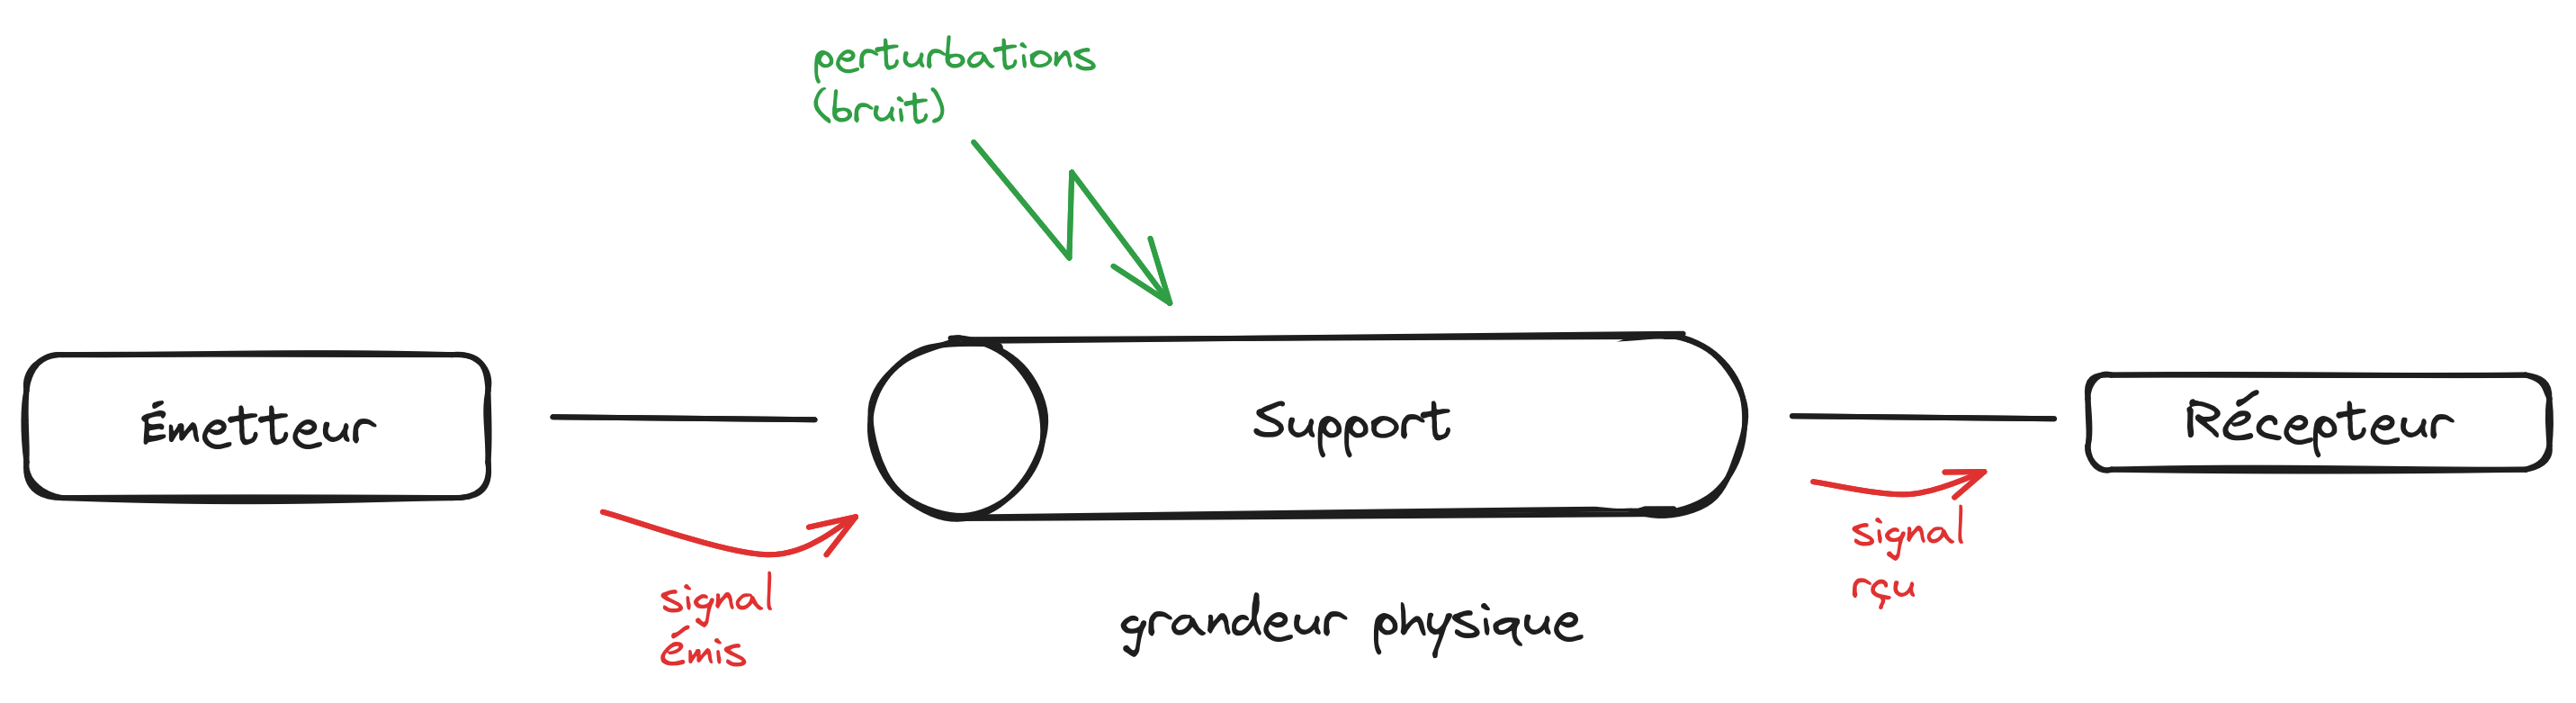
\includegraphics[width=1\linewidth]{imgs/support.png}
    \caption{Schéma représentatif d'un canal de transmission}
    \label{fig:canal}
\end{figure}

Un support de transmission admet une Bande passante \textbf{Bp}. Celle-ci est caractérisée par l'ensemble des fréquences que le canal permet de transporter. Ainsi que leur localisation dans l'espace des fréquences. Une bande passante admet donc une fréquence de début, une de fin, et une dernière centrale.
\\ \\
Bp de 100 Hz centrée sur 50 Hz. Soit Bp permet de transmettre toute fréquence dans l'intervale [0 Hz ; 100 Hz]
\\ \\
À leur dépassement à ses extrémités, le signal ne sera pas bien transmis; trop de dégradations seront appliquées pour les fréquences en dehors de la bande passante. Si nous pouvions avoir un canal de transmission parfait, avec aucune limite de bande passante et sans atténuation, alors le débit maximal théorique obtenable serait parfait aussi, outrepassant toute loi de la physique mais utile pour des calculs.
\\ \\
Ainsi, un canal de transmission avec une meilleure bande passante permet un meilleur débit binaire théorique : e.g. avec la fibre optique et une paire torsadée. Le signal "ne va pas plus vite", la vitesse de l'électricité dans un conducteur étant relativement proche de celle de la lumière dans du silice, mais la bande passante permise par le changement de support permet un meilleur débit, par la fibre moins d'atténuation, facilitant l'élargissement de la bande passante.
\\ \\
Dans la caractérisation de la chaîne de transmission du monde du numérique, nous avons rappelé le principe de liaison synchrone et asynchrone (synchronisation des horloges ou resynchronisation du front de décision à chaque information). Nous avons aussi revu le principe de débit binaire maximal théorique (brut), et celui dit "net" à l'utilisation - après toutes les informations nécessaires à la transmission des données ajoutées pour assurer sa transmission (dans les entêtes et queues des couches des protocoles).
\\ \\
Dans la caractérisation d'un signal, nous avons vu l'apparition des zones de décision pour différencier les états significatifs d'un signal. Pouvant se traduire par la plage de décision permise pour définir si l'on peut différencier un état significatif du signal (codant une information), pouvant laisser place à une zone d'incertitude. La place de décision doit toujours être inférieure au temps d'un état, sinon possibilité de confusion.

\begin{figure}[h]
    \centering
    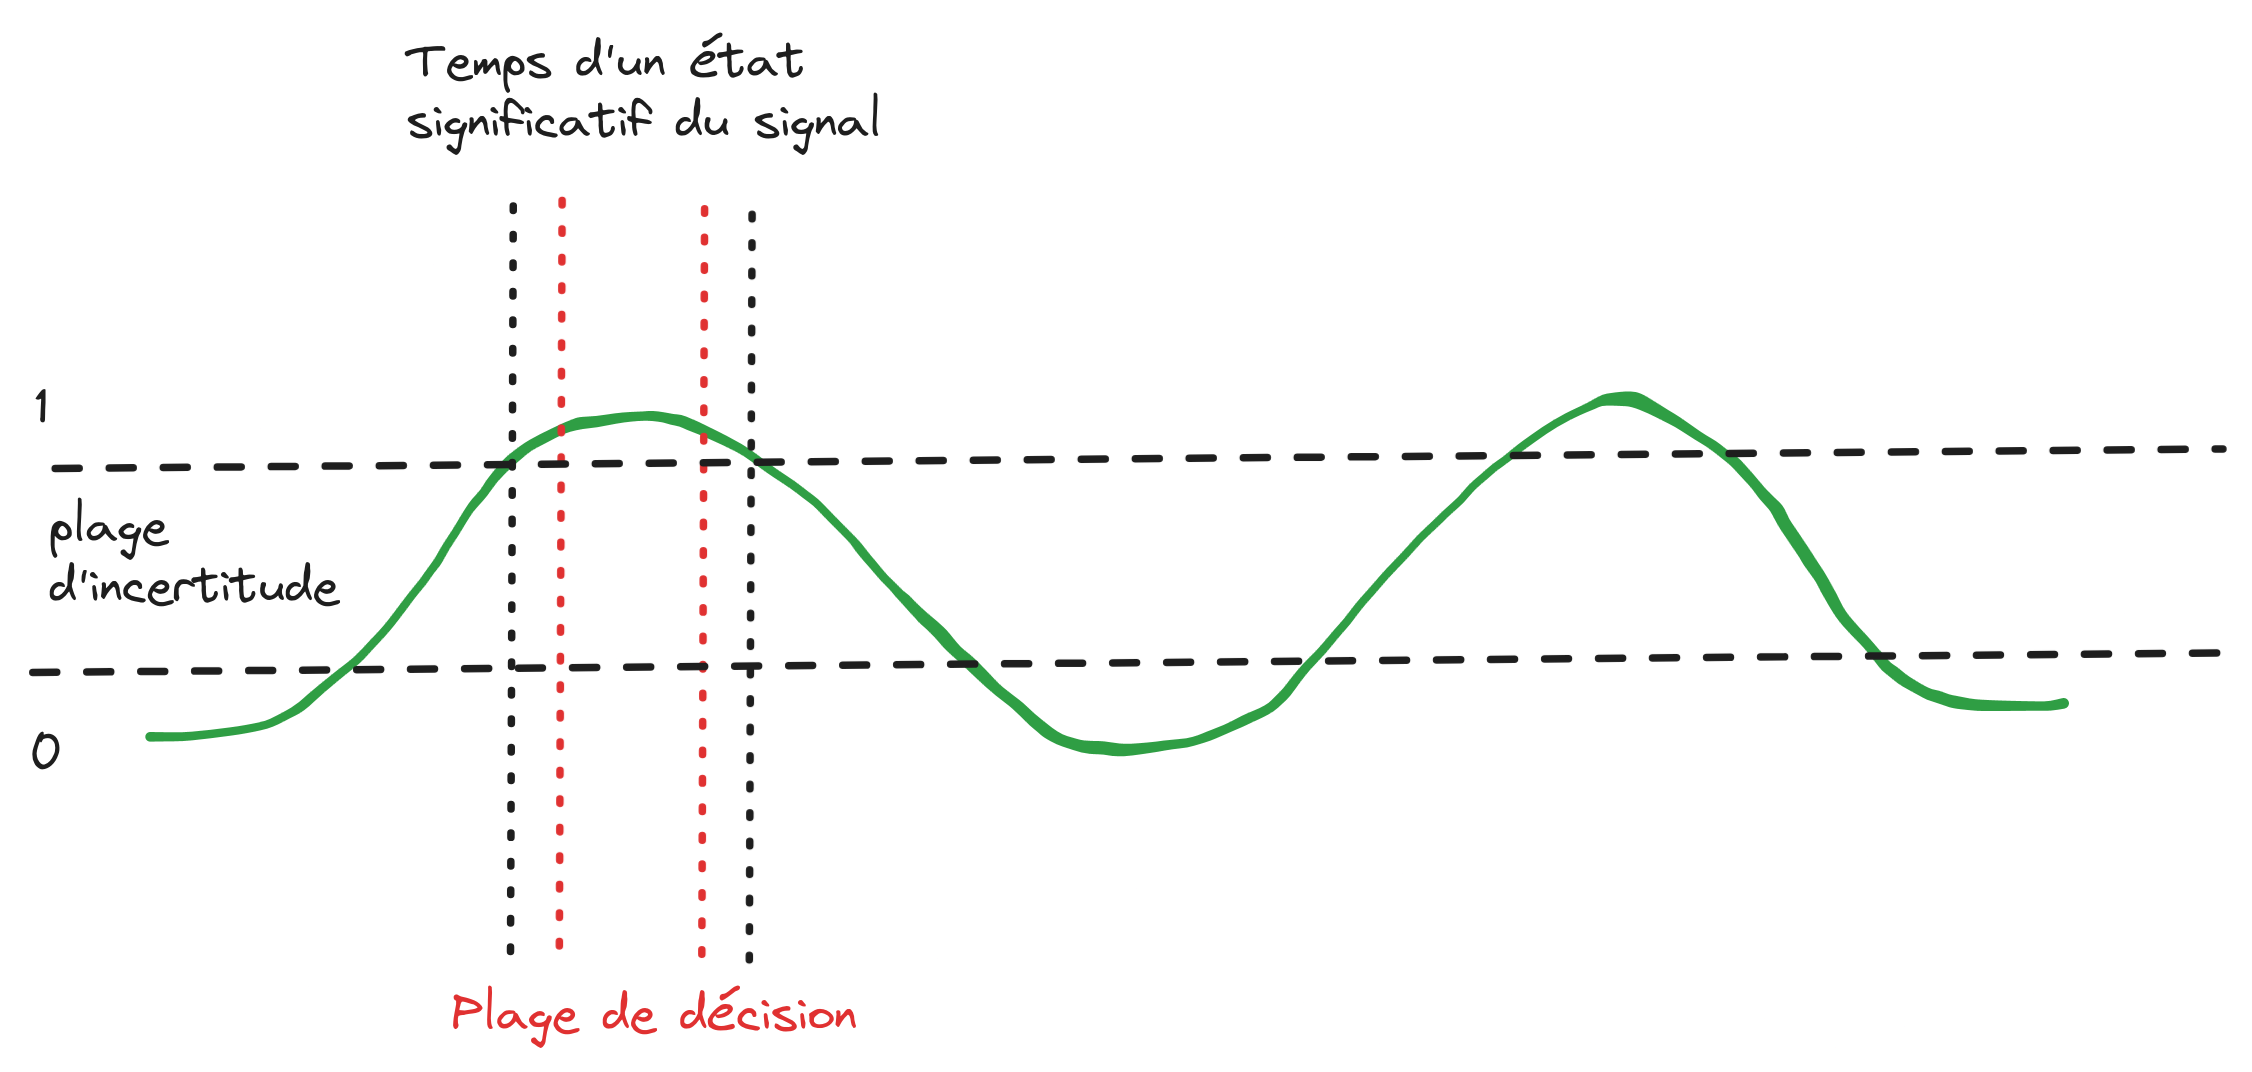
\includegraphics[width=1\linewidth]{imgs/td.png}
    \caption{Schéma représentatif de la décision d'un état pour une sinusoïde simple, ou "comment définir l'état d'un signal"}
    \label{fig:td}
\end{figure}

Par ce schéma, on peut en ressortir que si une plage de décision est trop large comparée au moment d'un symbole (état significatif d'un signal) : on peut confondre un état pour un autre. Il s'agit de l'interférance inter-symbole, ici représenté par deux états électriques +A -A (A pouvant être négatif). L'intérêt est de bien configurer les seuils de décisions (encadrement des valeurs du signal - plage d'incertitude) et les temps de décisions (plage de décision d'un moment).
\\ \\
Un autre moyen plus simple de mettre en évidence l'interférance inter-symbole est de diagramme de l'oeil. Dans celui-ci sont défini tous les passages possibles des états.

\begin{figure}[h]
    \centering
    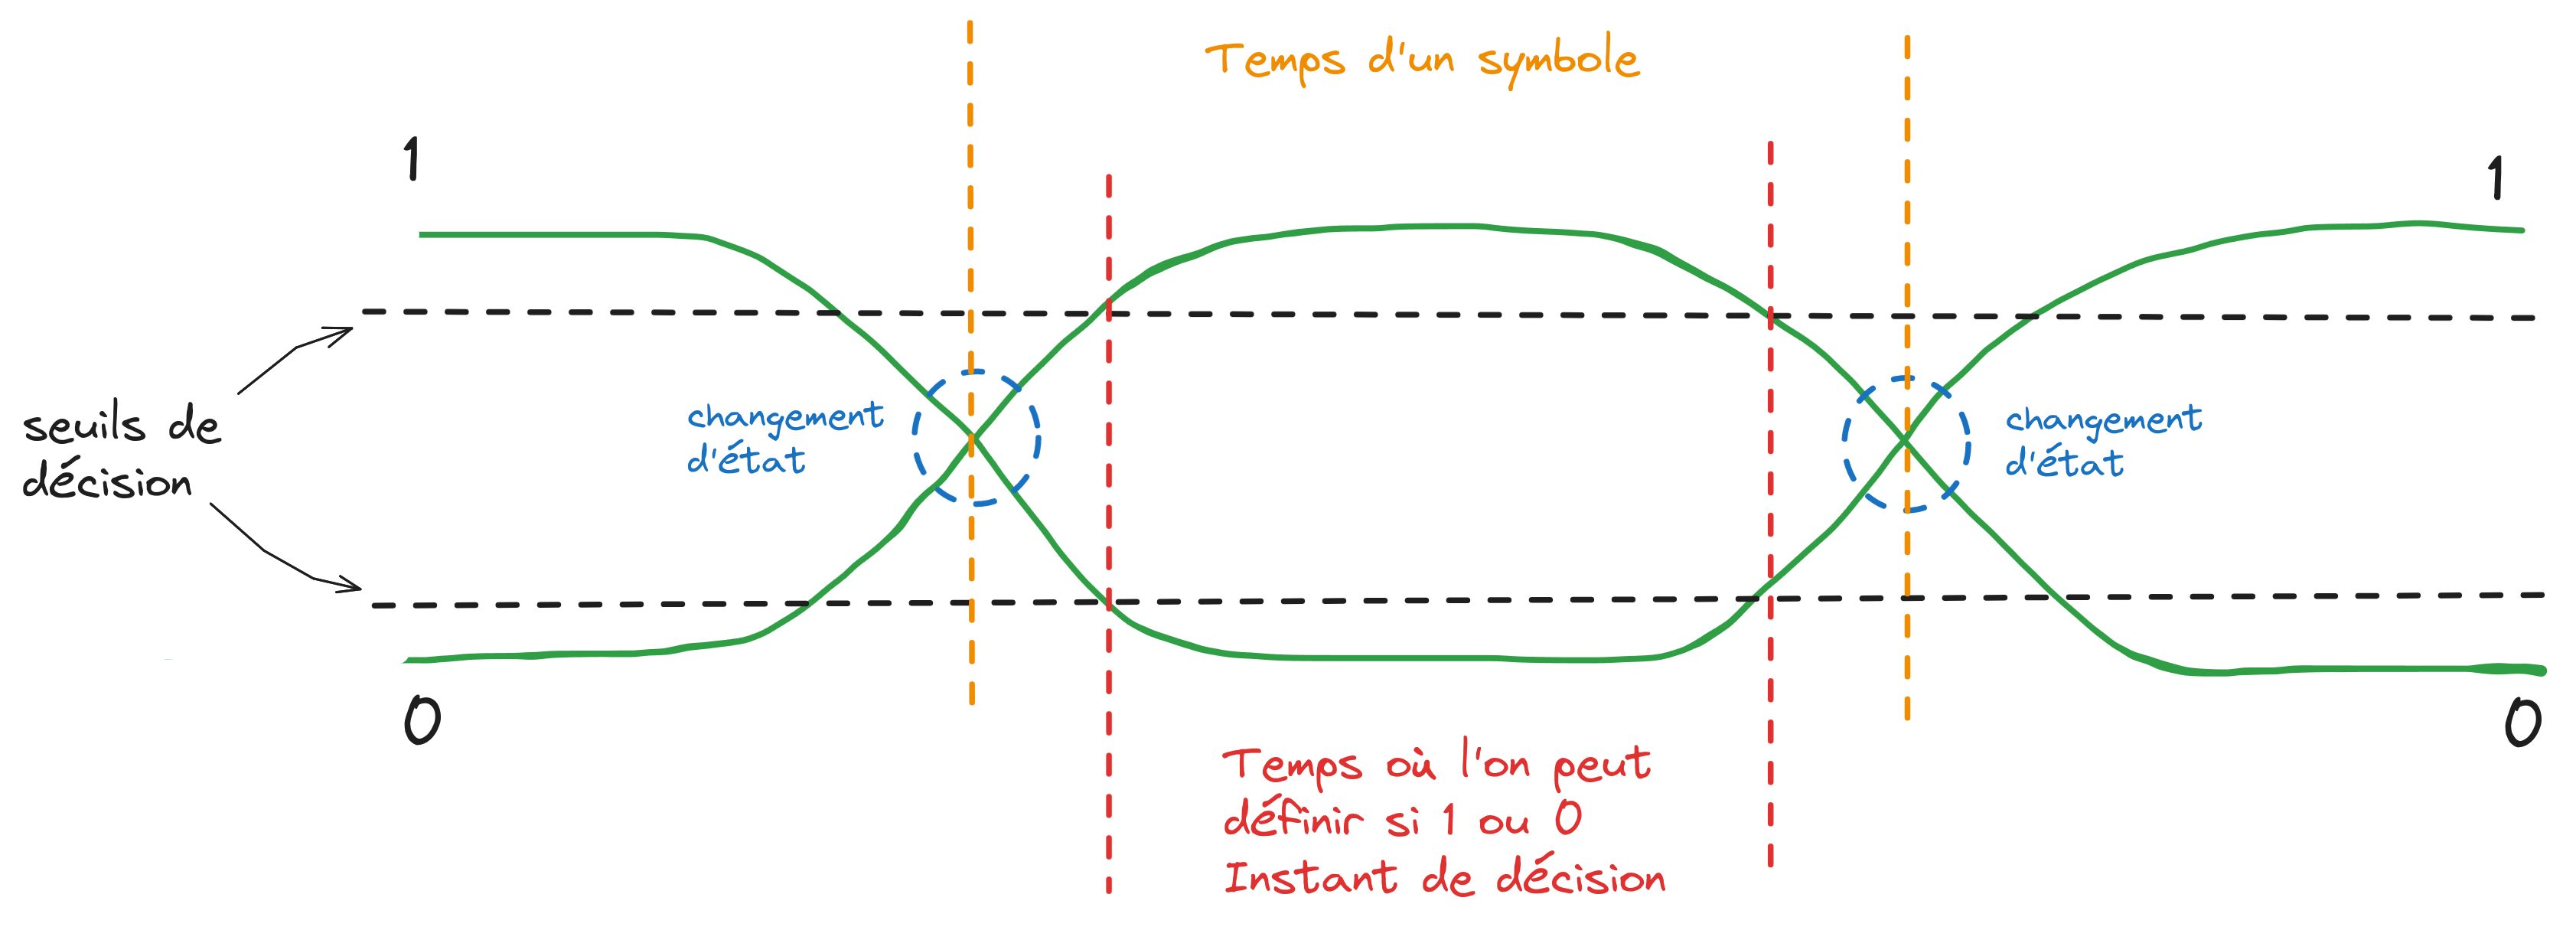
\includegraphics[width=1\linewidth]{imgs/seuils.png}
    \caption{Introduction au diagramme de l'oeil par identification des états d'un signal carré sans bruit (très fin)}
    \label{fig:seuils}
\end{figure}

Le temps où l'on peut définir si l'état est à 0 ou 1 ne peut être plus grand ou égale qu'à celui des symboles, sinon interférence inter-symbole. Le temps d'un symbole commence dès le changement du précédent état. Si l'instant de décision n'est pas correcte, deux choix pour atteindre les seuils si on ne peut pas les modifier : diminuer le débit pour faire rentrer le signal dans leur intervale, ou augmenter la bande passante - en changeant de canal de transmission.
%\\ \\
%Nous avons fait la différence entre le débit binaire brute théorique attégnable, et celui reçu après informations rajoutées aux données envoyées (destination dans un réseau, gestion de sessions, encapsulation de protocoles...) dans des entêtes et/ou des queues.
\\ \\
Nous pouvons changer le débit en conservant une bande passante correcte en jouant sur la valence du signal. En conservant la même fréquence, nous pouvons moduler le signal en amplitude ou en phase afin d'avoir davantage de symboles. La limite de cette pratique nous est donné par les travaux de Mr. Shanon que nous avons étudié, fixant que la valence se limite à ce que permet le rapport signal sur bruit, pour distinguer tous les états.
\\ \\
Nous avons aussi repris les travaux de Mr. Nyquist en intégrant ses critères pour définir la capacité d'un canal, soit sa bande passante maximale dans le domine théorique et physique. Nous avons notamment démontré la différence entre ces deux en travaux pratiques.
\\ \\
Si le débit binaire augmente, la bande passante aussi, sinon interférence entre les symboles. Pour contrer ceci soit augmenter la bande passante, soit réduire le débit, soit jouer sur les seuils et les instants de décision. D'autres états peuvent être introduits par modulation, à question que ceux-ci puissent être distingués, donc pas limités par le rapport entre le niveau de puissance du signal et celui du bruit.

\section{Fiabilisation d'une transmission}

La fiabilisation d'une transmission peut se caractériser par sa capacité à transmettre un message selon des circonstances données. Ainsi, des mécanismes de contrôle d'erreurs sont instaurés avec une demande de ré-émission par exemple. Le choix du type de transmission est aussi important, sa modulation. Dans cette partie nous avons abordé les codecs et nous avons étudié les types de modulation (manchester, NRZ...).
\\ \\
Certains types de modulations permettent une meilleur résistance au bruit, notamment ceux par phase vu diagramme de constellation. Chacun code le signal comme il le souhaite, le temps et les chercheurs sont par exemple passés du codage NRZ \textit{non-return-to-zero} à du PSK \textit{Phase-shift keying} ou du QAM \textit{quadrature amplitude modulation} toujours utilisés aujourd'hui. Leur largeur de spectre pour les mêmes informations envoyées changent aussi, pareil que pour son emplacement dans un spectre d'amplitude (lobe principal centré sur 0 Hz pour ceux qui ne modulent pas en fréquence...).

\section{Aboutissants du module}

Nous avons approfondi nos connaissance dans les supports de transmissions qui nous servent aujourd'hui. Nous pouvons les caractériser correctement pour montrer une infrastructure, nous pouvons les diagnostiquer dans nos domaines de compétences. Nous comprenons désormais comment circule un signal dans la "chaine du transmission du numérique", son histoire et son arrivée au monde moderne.
    \renewcommand{\figurename}{}
\mychapter{R3.06 Fibres optiques et propagation (19h30)}{cap:r306} 
\lhead{R3.06 Fibres optiques et propagation (19h30)}
% wdm
% longueur d'onde
% utilisation réflectomètre
% zone aveugle, zone morte
% différentiation atténuation coupleur, connecteurs, épissure

\vspace*{0.2cm}%
      \large
      \href{}{\color{black}Enseignant\\M. Christophe Baillot}\\%
      \normalsize
\vspace*{0.5cm}%

Beaucoup de notions sur la fibre optique en travaux pratiques et théoriques ont été abordées durant ces 19h30. Nous avons principalement vu les applications des domaines physiques apportés par la fibre optique (fonctionnement de la lumière dans l'infrastructure fibre actuelle) et quelques applications avancées (multiplexage d'ondes, utilisation d'un réflectomètre).

\section{Apprentissages théoriques}

En cours magistraux et lors des travaux dirigés, nous avons compris le fonctionnement de la lumière dans du silice actuellement utilisé, ses avantages sur les autres technologies de transport du signal et son application par des calculs. Le fonctionnement de la fibre optique se comprend en \textbf{longeur d'onde}, où une longeur d'onde est envoyée dans un noyau de silice (verre) et y est comprise à l'autre extrémitée.
\\ \\
La vitesse de la lumière dans du silice et celle de l'électicité dans du cuivre sont contre-intuitivement relativement proches. La lumière n'est pas \textit{"plus rapide"} que l'électricité : la réponse à son écrasante supériorité réside dans le fait qu'aucune fréquence n'est assez élevée pour venir perturber la longeur d'onde transmise dans le support (pas de perturbation commesur du cuivre, de bruit). La lumière est aussi moins réceptive à l'atténuation.
\\ \\
La lumière rencontre cependant de l'atténuation qui survient lorsque sont reliés deux extrêmités de silice. Dans un diagramme de perturbation de la fibre optique relevé par un réflectomètre, nous avons appris à observer les différentes causes d'atténuation.

\begin{figure}[H]
      \centering
      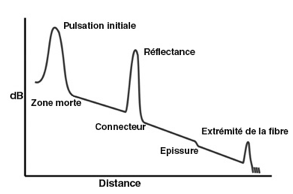
\includegraphics[width=\textwidth - \textwidth / 5]{ressources/r306/00.png}
      \caption{Le signal faiblit naturellement avec la distance. La zone morte correspond à la zone de non visibilité de l'appareil (la lumière étant trop forte pour y dicerner quelque chose, plus on émet fort). Un connecteur (comme une prise) fait joindre verticalement ou horizontalement pour les plus récents deux jartières ("câbles") : la lumière rencontre un obstacle car de l'air est entre et y est réfléchie, ce qui provoque une réflectance et une augmentation du niveau de puissance reçue pour l'appareil. Une épissure est une jonction soudée de deux noyaux de silice.}
      \label{fig:r306-00}
\end{figure}

Ce diagramme a été fait sur une longeur d'onde, mais il pourrait être applicable sur d'autres longueurs d'ondes fréquemment utilisées. Celles-ci sont différenciées selon si elles sont utilisées pour des fibres dites monomode (1310 nm et 1550 nm) à un seul chemin ou multimodes (850 nm et 1300 nm) à chemins multiples. Ces longeurs ont été choisies car l'atténuation y est moins importante pour la lumière. La fibre monomode est souvent préférée aujourd'hui.
\\ \\
Beaucoup d'autres notions ont été abordées : cône d'acceptance, fibres multimode à gradient d'indice, protocole GPON...

\section{Apprentissages pratiques}

Nous avons pu manipuler lors des séances de travaux pratiques des réflectomètres et des fibres optiques afin de monter et caractériser nos premières liaisons.
\\ \\
Un réflectomètre est un appareil de mesure permettant de caractériser le passage de la lumière dans une fibre optique pour s'assurer de son intégrité. Nous avons revu avec eux la différence entre zone morte et zone aveugle, les atténuations générées par les manipulations humaines et tout l'importance de changer la longueur d'onde envoyée selon la distance que l'on souhaite observer.

\begin{figure}[H]
      \centering
      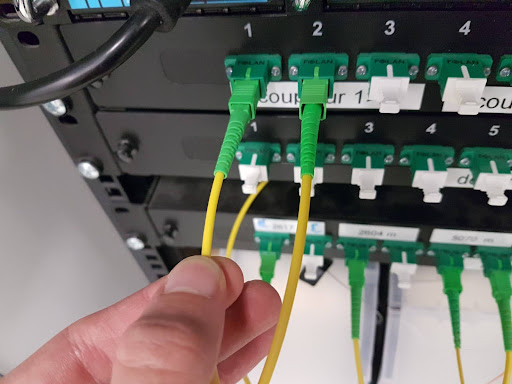
\includegraphics[width=\textwidth - \textwidth / 5]{ressources/r306/01.jpg}
      \caption{Utilisation de l'infrastructure de la salle pour simuler nos premières fibres.}
      \label{fig:r306-01}
\end{figure}

Nous avons aussi vu la technologie WDM. Contrairement aux fibres monomodes qui transportent une longeur d'onde mais en empruntant plusieurs chemins; WDM permet de faire circuler plusieurs longeurs d'ondes, donc plusieurs informations, dans le même support. Cette technologie est extrêmement utilisé dans les coeurs de réseaux opérateur.

\begin{figure}[H]
      \centering
      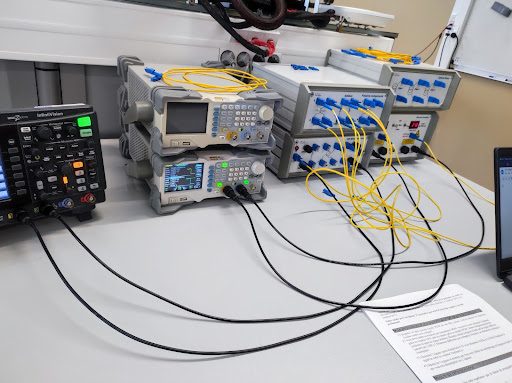
\includegraphics[width=\textwidth - \textwidth / 5]{ressources/r306/00.jpg}
      \caption{Mise en place et caractérisation d'une structure WDM en travail pratique.}
      \label{fig:r306-02}
\end{figure}
    \renewcommand{\figurename}{}
\mychapter{R3.09 Programmation événementielle (15h)}{cap:r309} 
\lhead{R3.09 Programmation événementielle (15h)}
    \renewcommand{\figurename}{}
\mychapter{R3.11 Anglais : le monde du travail (22h30)}{cap:r311} 
\lhead{R3.11 Anglais : le monde du travail (22h30)}

\vspace*{0.2cm}%
      \large
      \href{}{\color{black}Enseignant\\Jeff}\\%
      \normalsize
\vspace*{0.5cm}%

Jeff de son surnom, est notre professeur d'anglais lors de cette deuxième année. Son objectif était de réhausser notre niveau en grammaire et à l'oral pour passer au mieux des examens d'anglais écrits ou des oraux; pour intégrer des écoles d'ingénieurs, nous entainer ou valider notre niveau d'anglais pour de futurs entretiens. 

\section{Grammaire}

Nous avons revu avec Jeff des notions importantes de grammaire anglaise pour le passage d'examens écrits tel que le TOEIC pour valider notre niveau de maitrise. Ce qui nous a conduit à revoir notre formulation, trop courrante ou non adaptée.
\\ \\
L'apprentisasge se faisait par le biai de QCM \textit{Questionnaires à Choix Multiples}, pareil pour l'examen.

\section{Passages à l'oral}

Nous avons aussi travaillé notre prononciation et notre aisance à l'oral en proposant des présentations devant notre classe. Jeff nous donnait un choix de sujet (notre enfance ici) et nous demandait de passer à l'oral sans durée déterminée en nous jugeant sur notre grammaire, notre capacité à répondre aux questions et notre attitude.
    \renewcommand{\figurename}{}
\mychapter{R3.14 Mathématiques: Analyse de Fourier (27h)}{cap:r314} 
\lhead{R3.14 Mathématiques: Analyse de Fourier (27h)}
    \mychapter{Annexes}{cap:annexes}
\lhead{Annexes}

Regroupement des documents servant à l'appui des éléments cités précédemment. Pouvant être de toutes formes (images, blocs de texte, photos...).

\section{Cahier des charges supervision}

Cahier de charges supervision

La recherche de solution applicative de supervision devra se base au
minimum sur deux applications pour avoir une comparaison objective.

Voici les fonctionnalités souhaitées~:

\ul{Serveurs Proxy}

L'utilisation de \textbf{SERVEUR PROXY} pour ne pas avoir un seul
serveur qui se charge de l'ensemble de vérifications de sonde.

\ul{DASHBOARD}

Un \textbf{DASHBOARD UNIQUE} qui inclut l'ensemble des serveurs de
supervision.

\ul{DASHBOARD TV}

Un \textbf{DASHBOARD} pour la télé qui liste les notifications de la
plus récente a la plus ancienne. (Comme celle que l'on a actuellement.)

\ul{Type de contrôles}

L'application devra gérer les contrôles \textbf{PASSIF} et
\textbf{ACTIF} et la prise en charge des contrôles via \textbf{SNMP}.

\ul{Type de paramétrages}

La possibilité de configurer les hosts via l'interface graphique et via
les fichiers de configuration.

Exemple~: sur l'ancienne supervision on créer un fichier de conf par
client.

\ul{Notifications}

Les notifications devront être effectuées par mail et par SMS tout en
ayant une gestion des utilisateurs et des groupes (possibilité
d'intégrer la solution à notre serveur d'SMS)

Déplacer le GSM dans le bureau ADITU de Pulseo pour une meilleur
couverture réseau (prévoir onduleur + switch mangeable)

\ul{Accès restreint client}

Donner la possibilité à certains clients de visionner leur supervision
en lecture et d'être alerté par mail.

\ul{Graphique}

Côté graphique, il serait bien que la solution puisse avoir la
possibilité d'inclure les graphiques comme fait Cacti pour éviter
d'avoir 2 solutions.

\begin{itemize}
\item
  Graphique réseau
\item
  Graphique volumétrie disque pour voir l'évolution du stockage
\item
  Graphique mémoire ou CPU
\end{itemize}

\ul{Tarif}

Open source gratuit

% \begin{figure}[H]
%     \centering
%     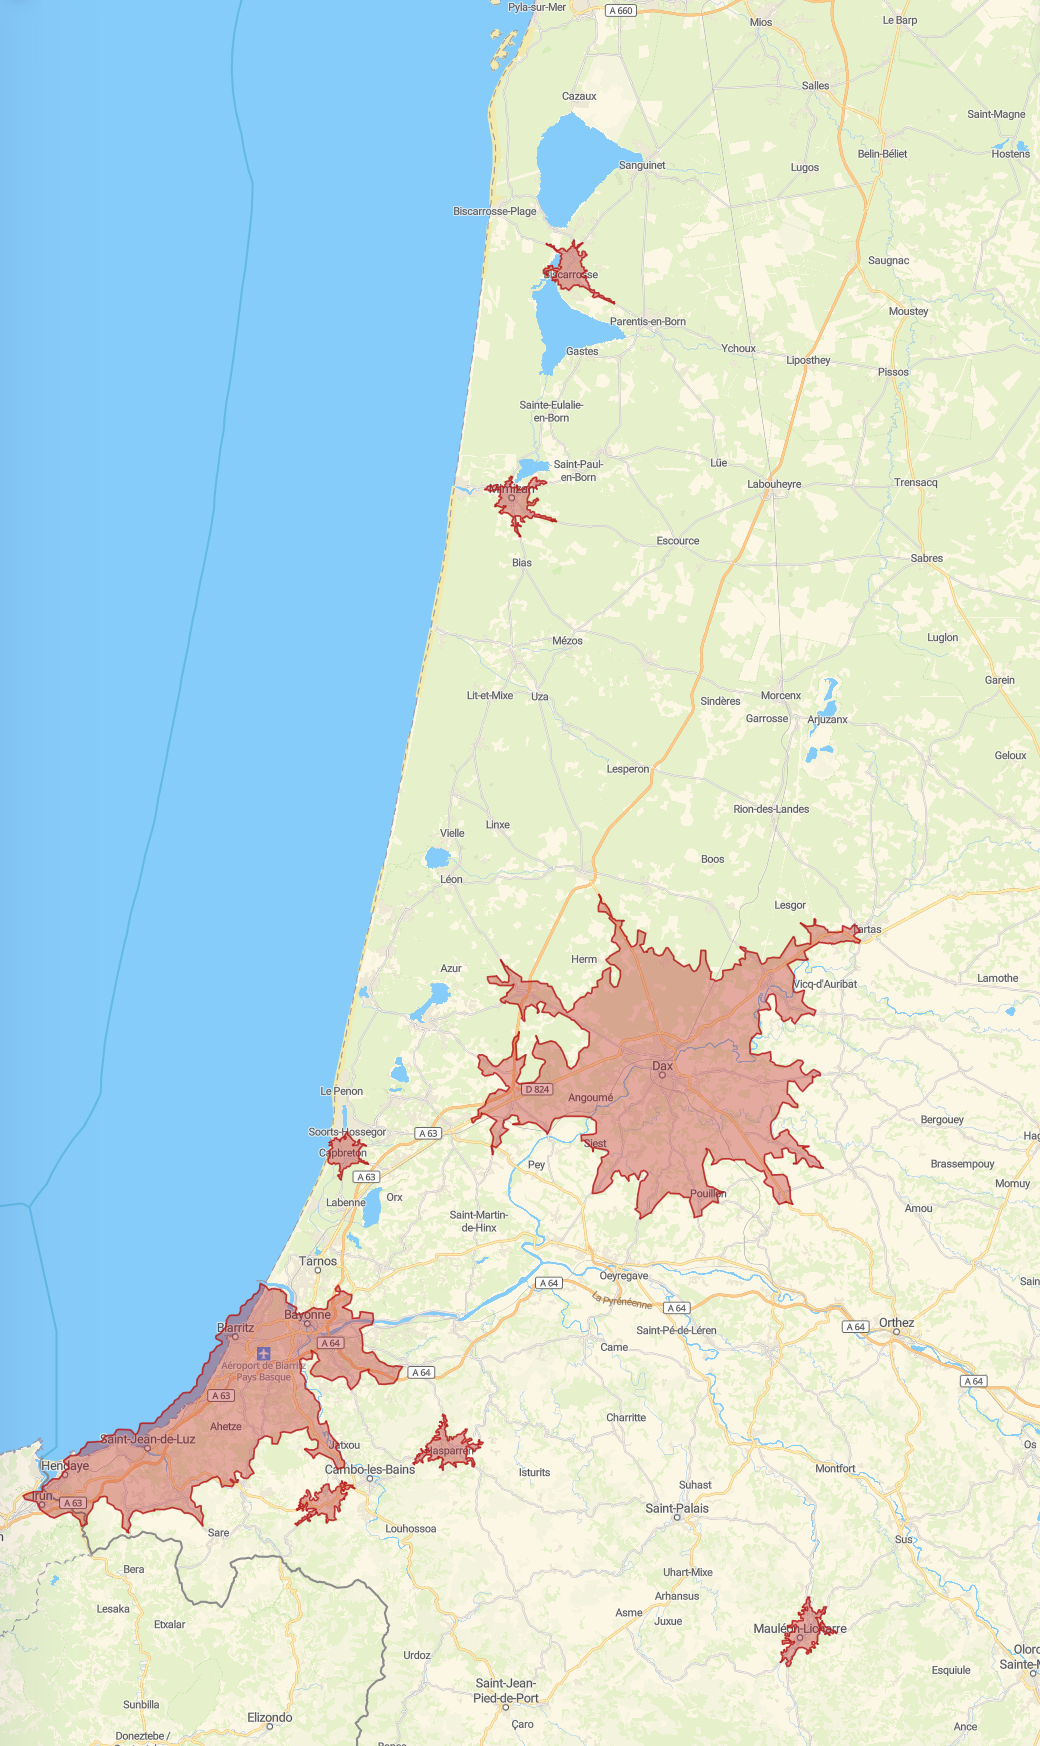
\includegraphics[width=\textwidth - \textwidth / 5]{zone_chalandise_aditu.png}
%     %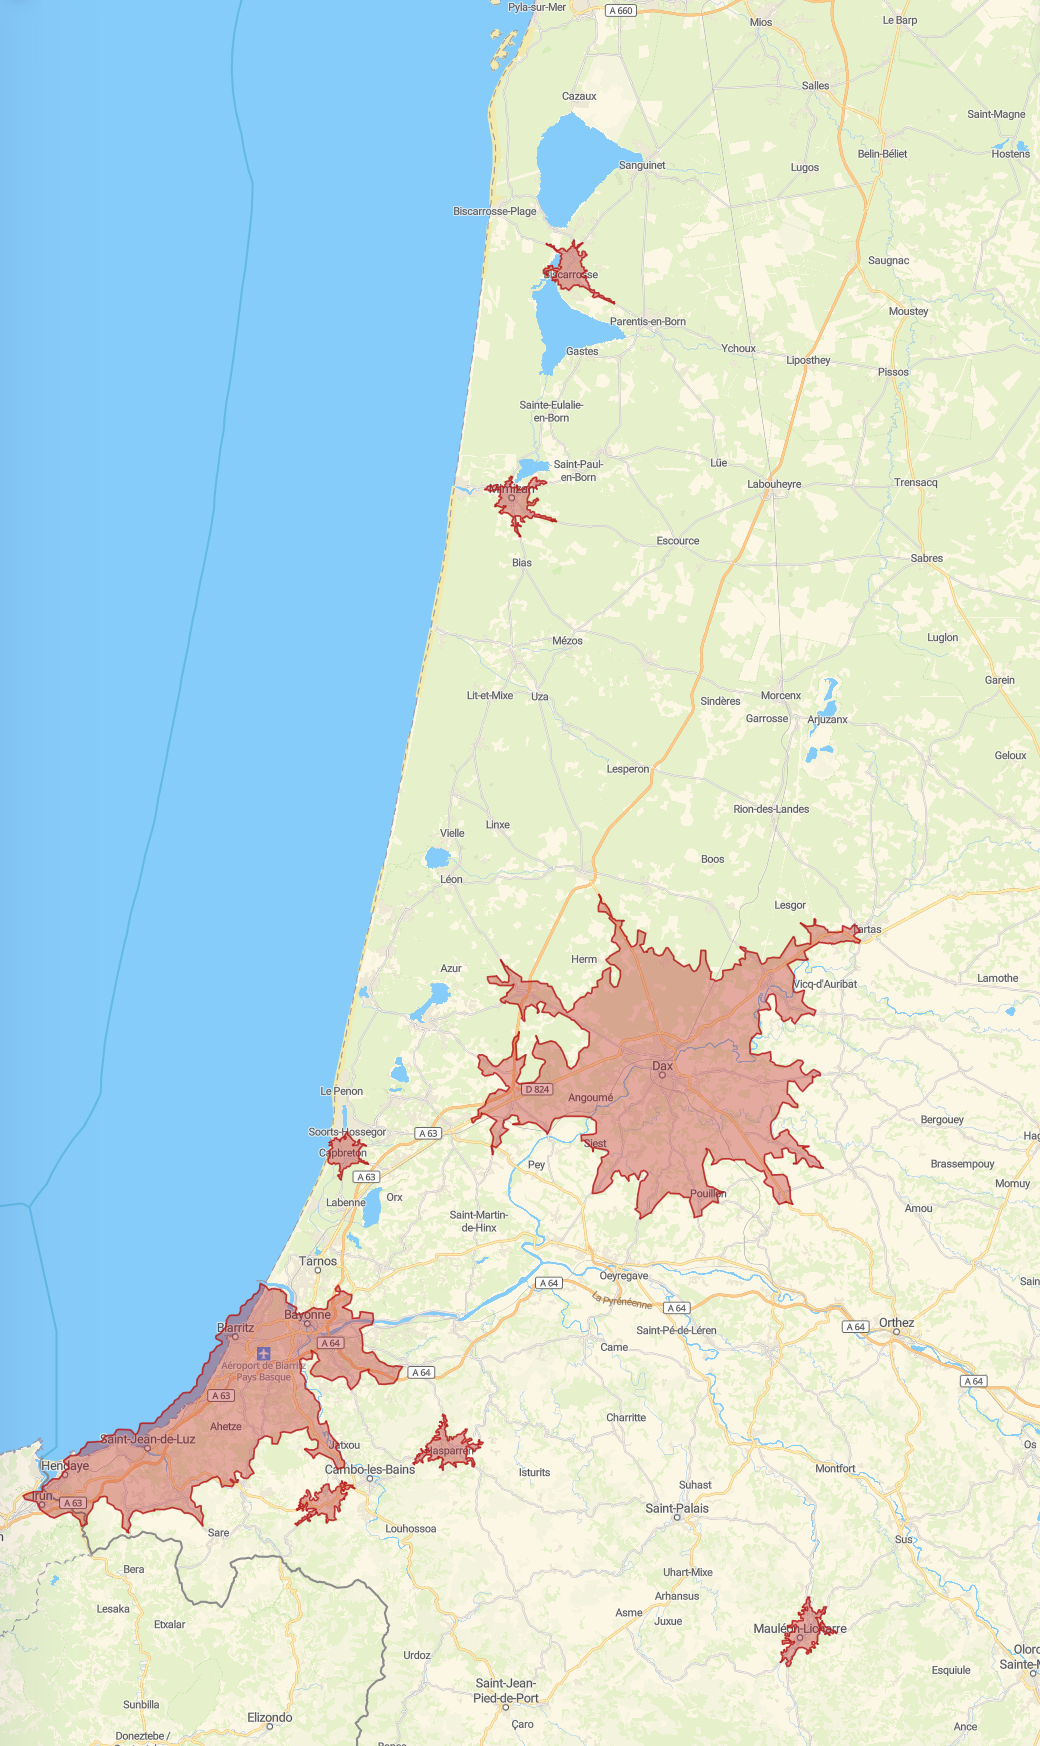
\includegraphics[scale=0.2]{zone_chalandise_aditu.png}
%     \figurename
%     \caption{Visualisation de la zone de chalandise d'ADITU, regroupée autour de ses datacenters à Bidart et à Dax}
%     \label{fig:zone_chalandise}
% \end{figure}

% \section{Cahier des charge Ticketing}

% % \begin{figure}[H]
% %     \centering
% %     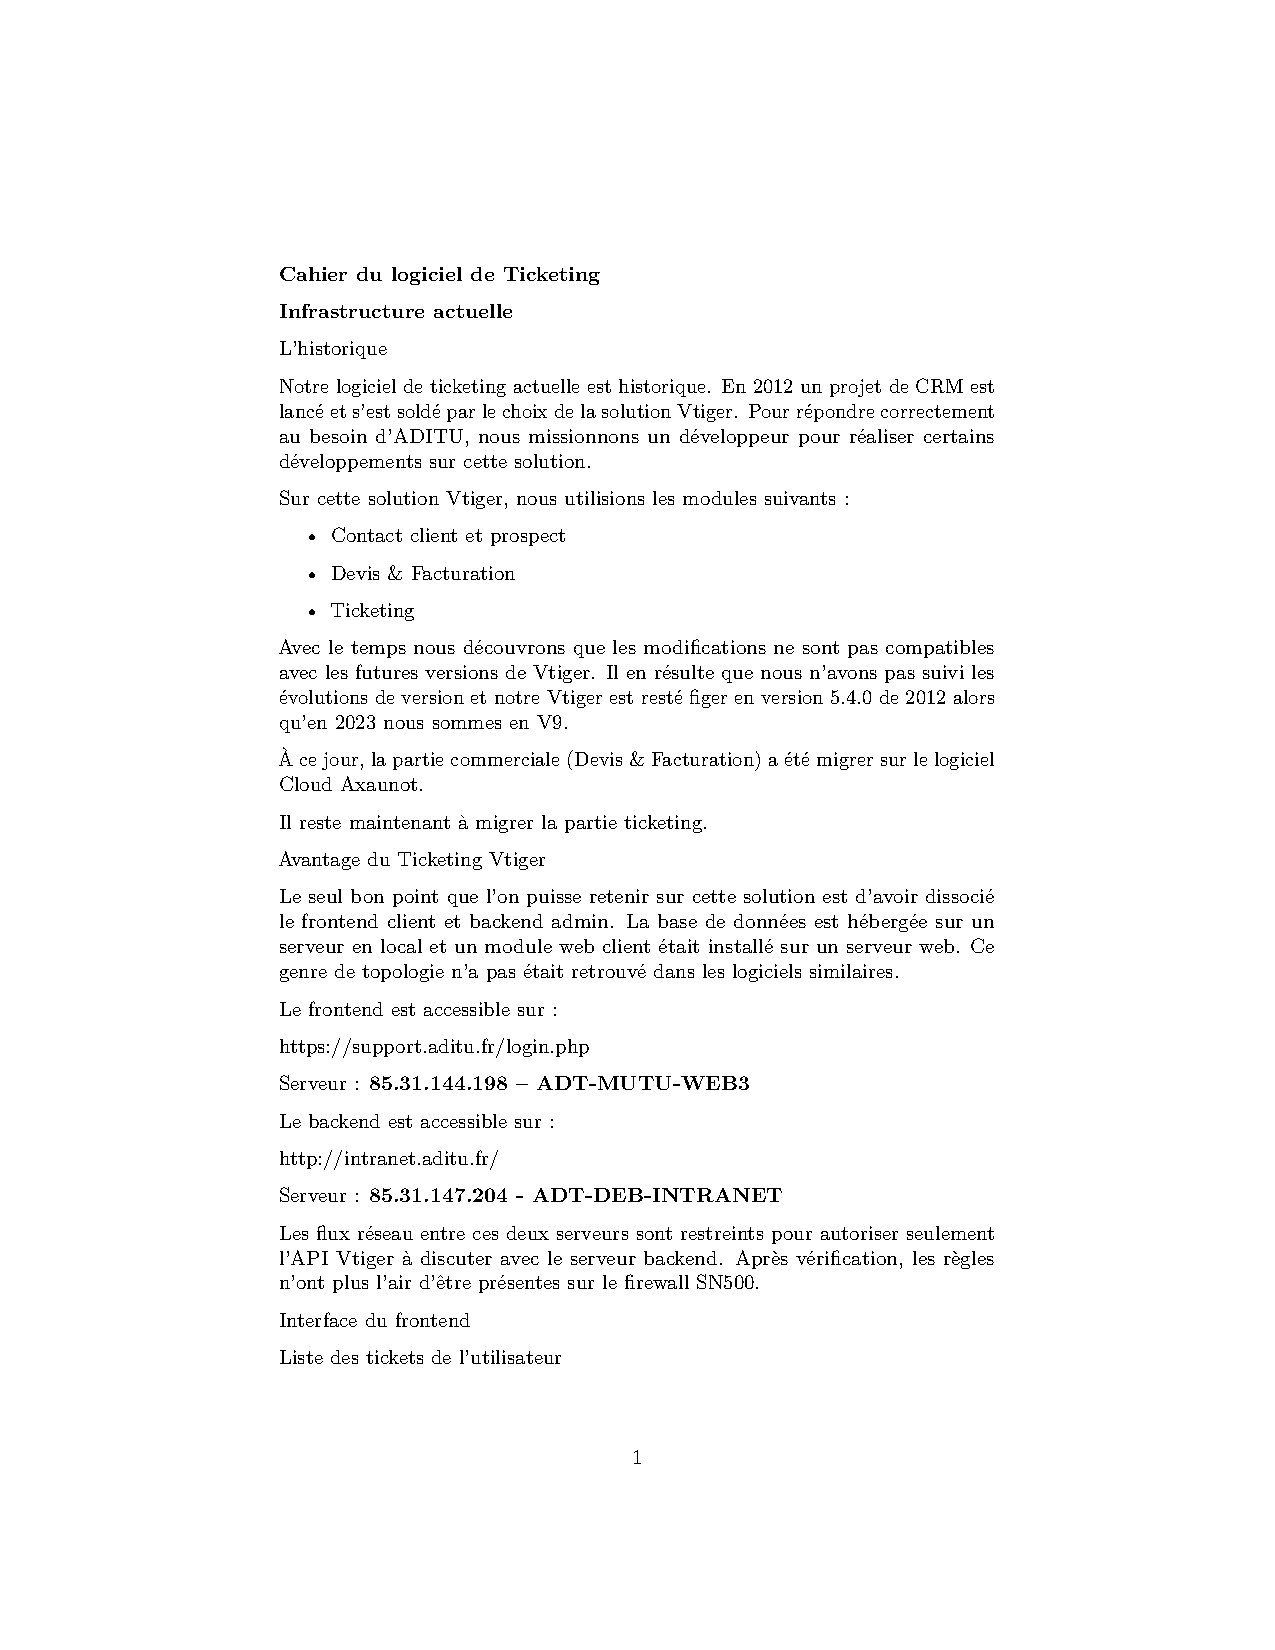
\includegraphics[width=\textwidth - \textwidth / 20]{CDC-Ticketing.pdf}
% %     \figurename
% %     \caption{Fiche de poste de notre alternance}
% %     \label{fig:poste}
% % \end{figure}

% \textbf{Cahier du logiciel de Ticketing}

% \textbf{Infrastructure actuelle}

% L'historique

% Notre logiciel de ticketing actuelle est historique. En 2012 un projet
% de CRM est lancé et s'est soldé par le choix de la solution Vtiger. Pour
% répondre correctement au besoin d'ADITU, nous missionnons un développeur
% pour réaliser certains développements sur cette solution.

% Sur cette solution Vtiger, nous utilisions les modules suivants~:

% \begin{itemize}
% \item
%   Contact client et prospect
% \item
%   Devis \& Facturation
% \item
%   Ticketing
% \end{itemize}

% Avec le temps nous découvrons que les modifications ne sont pas
% compatibles avec les futures versions de Vtiger. Il en résulte que nous
% n'avons pas suivi les évolutions de version et notre Vtiger est resté
% figer en version 5.4.0 de 2012 alors qu'en 2023 nous sommes en V9.

% À ce jour, la partie commerciale (Devis \& Facturation) a été migrer sur
% le logiciel Cloud Axaunot.

% Il reste maintenant à migrer la partie ticketing.

% Avantage du Ticketing Vtiger

% Le seul bon point que l'on puisse retenir sur cette solution est d'avoir
% dissocié le frontend client et backend admin. La base de données est
% hébergée sur un serveur en local et un module web client était installé
% sur un serveur web. Ce genre de topologie n'a pas était retrouvé dans
% les logiciels similaires.

% Le frontend est accessible sur~:

% \url{https://support.aditu.fr/login.php}

% Serveur~: \textbf{85.31.144.198 -- ADT-MUTU-WEB3}

% Le backend est accessible sur~:

% \url{http://intranet.aditu.fr/}

% Serveur~: \textbf{85.31.147.204 - ADT-DEB-INTRANET}

% Les flux réseau entre ces deux serveurs sont restreints pour autoriser
% seulement l'API Vtiger à discuter avec le serveur backend. Après
% vérification, les règles n'ont plus l'air d'être présentes sur le
% firewall SN500.

% Interface du frontend

% Liste des tickets de l'utilisateur

% 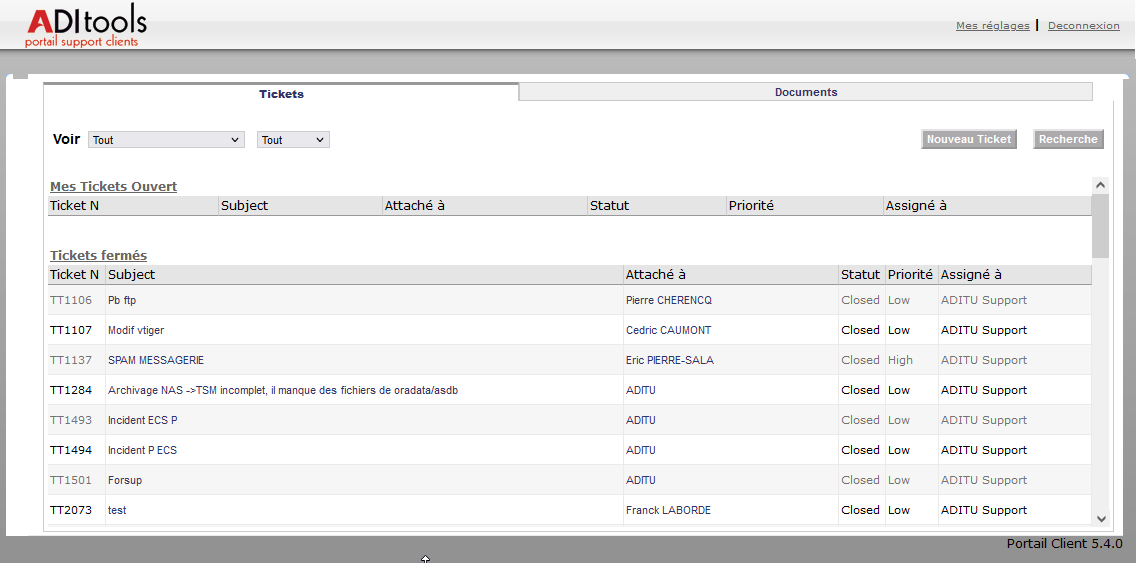
\includegraphics[width=6.3in,height=3.12222in]{image1.png}

% Création de tickets

% 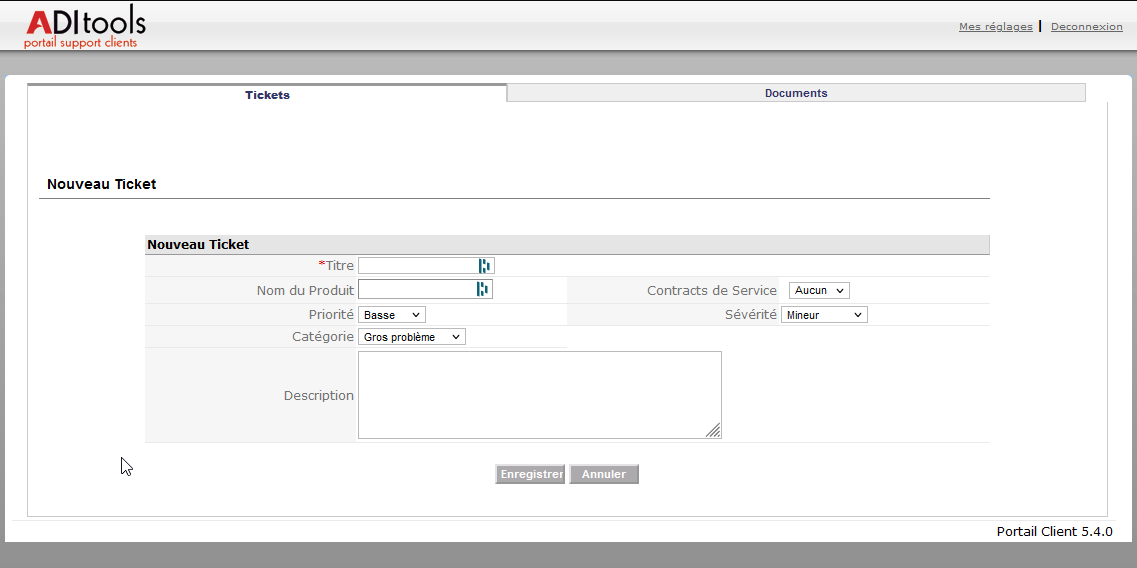
\includegraphics[width=6.3in,height=3.14722in]{image2.png}

% On peut constater que l'interface est plutôt minimaliste et
% vieillissante. Il manque certaines fonctions qui seront abordées plus
% bas.

% \textbf{Nouveau logiciel souhaité}

% Nous souhaitons migrer vers un nouveau logiciel de ticketing qui puisse
% intégrer les fonctionnalités ci-dessous~:

% Création d'incidents

% \begin{quote}
% La gestion des incidents permet de suivre et de résoudre les incidents
% signalés par les utilisateurs.
% \end{quote}

% Création de demandes de changement

% \begin{quote}
% Gestion des changements permet de planifier, suivre et gérer les
% modifications demandées par les utilisateurs.

% Exemple~: modification de ports sur le firewall, augmenter une boite aux
% lettres, etc.
% \end{quote}

% Création de tickets automatiquement

% \begin{quote}
% Cette fonctionnalité permet de planifier des interventions récurrentes
% sans les oublier. Exemple~: test de restauration
% \end{quote}

% Gestion des ressources

% \begin{quote}
% Pouvoir lié du matériel ou logiciel a un client et faire un suivi des
% modifications sur ce cette ressource.

% Exemple~: avoir le suivi des modifications comme celui qui est présent
% sur la page client du wiki.

% Intégrer du matériel lié à un fournisseur et gérer sa garantie. Exemple
% NAS ANANDA.

% Gérer les renouvellements~: des certificats

% Gérer les renouvellements~: des noms de domaines
% \end{quote}

% Inventaires

% \begin{quote}
% Lister l'ensemble des machines (connecteur OCS)
% \end{quote}

% Tableaux de bord et rapports

% Avoirs des stats et indicateurs sur ce qui nous prend le plus de temps
% dans le support.

% Ergonomique

% \begin{quote}
% Il faut que le logiciel soit intuitif et ergonomique. Que l'utilisateur
% ne soit pas rebuté par la complexité d'ouverture d'un ticket.
% \end{quote}

% Ouverture de ticket via email

% Fermeture de ticket automatique après un délai de non-réponse

% Personnalisation graphique

% \begin{quote}
% Nous souhaitons que l'application puisse se personnaliser aux couleurs
% de la société et d'y insérer le logo.
% \end{quote}

% Récupération des données ticketing vtiger

% \begin{quote}
% Seulement si cette récupération est facile. Ne pas perdre du temps sur
% cette récupération.
% \end{quote}

% Fonctions annexes

% Gestion des baies racks du datacenter


    % Pós Textuais
    % \nocite{*}
    % \include{pos-textuais/referencias}

\end{document}
